\chapter{Приложения и калибровка}
\section{Вольтметр}
Показывает напряжение аккумулятора во время работы. evo\_v\_l выводит числовое значение и значок аккумулятора; iv\_evo\_v\_t использует сегментное отображение, похожее на IV-Nano.

\begin{figure}[H]
\centering
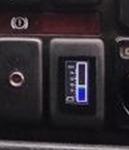
\includegraphics[width=.85\textwidth,height=.60\textheight,keepaspectratio]{figures/ivevo/image16.png}
\caption{Вольтметр}
\end{figure}

\begin{figure}[H]
\centering
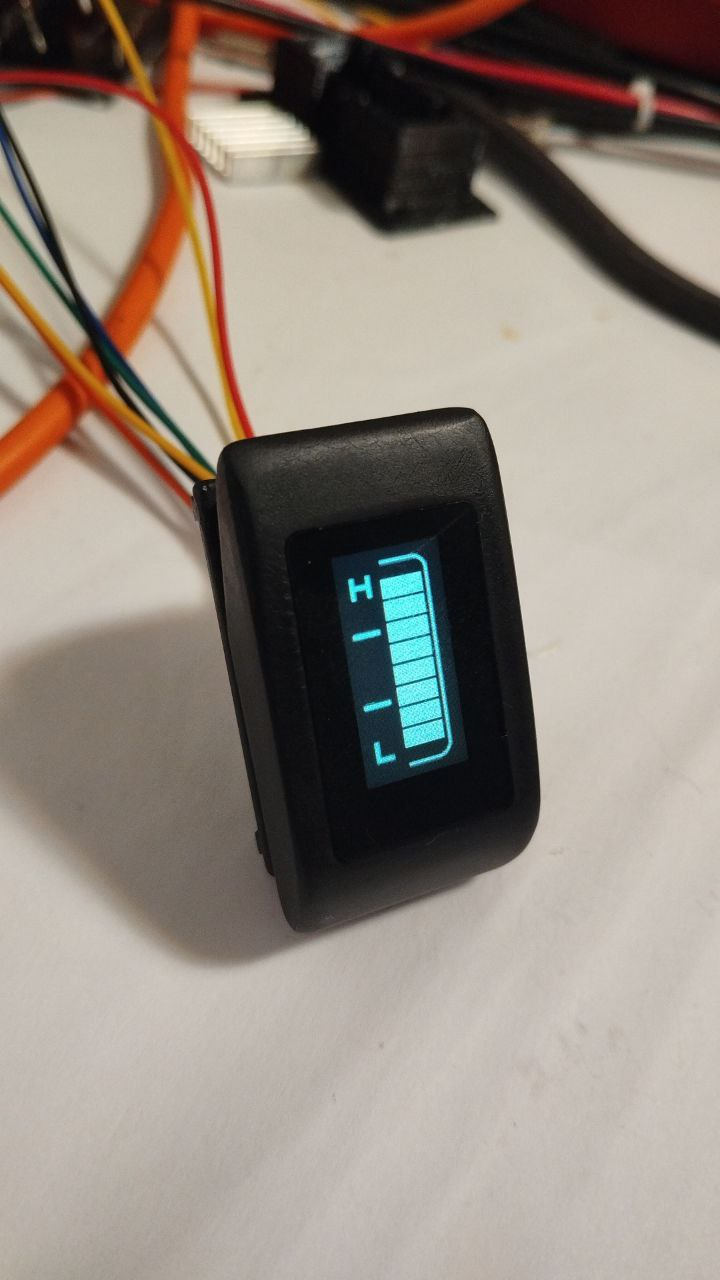
\includegraphics[width=.85\textwidth,height=.60\textheight,keepaspectratio]{figures/ivevo/image15.png}
\caption{Вольтметр}
\end{figure}

\begin{figure}[H]
\centering
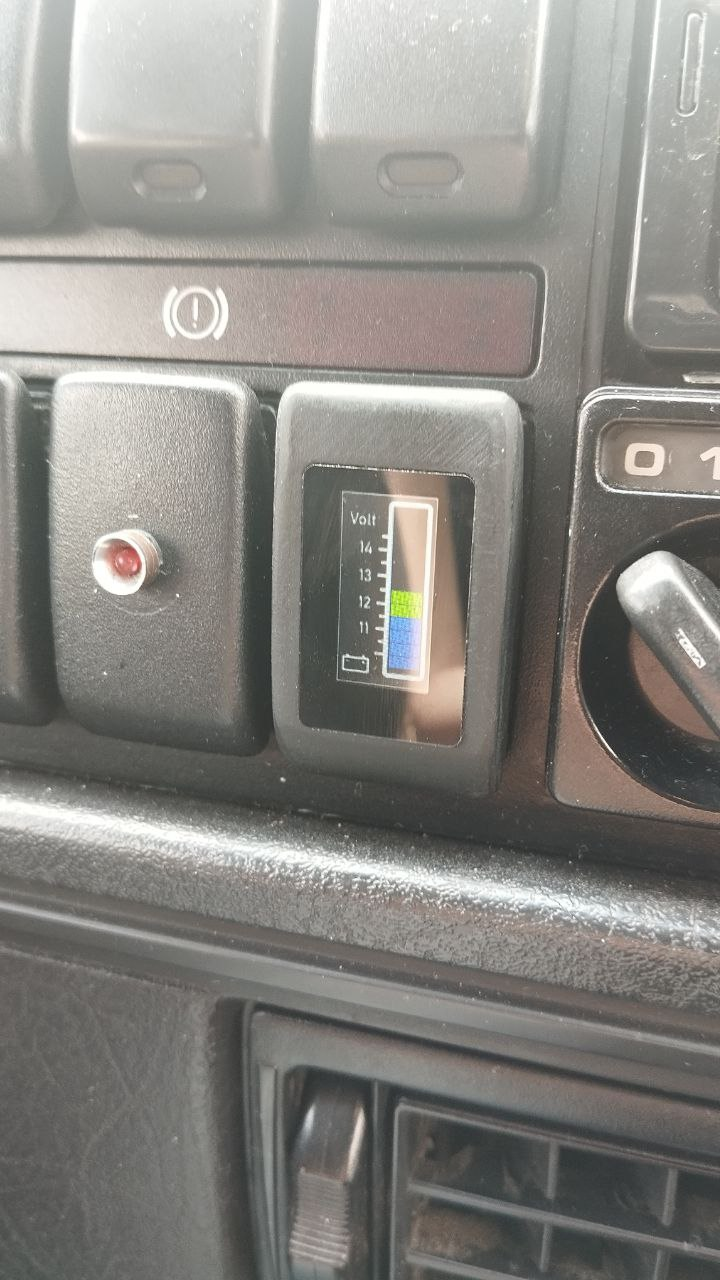
\includegraphics[width=.85\textwidth,height=.60\textheight,keepaspectratio]{figures/ivevo/image2.png}
\caption{Вольтметр}
\end{figure}
\section{Давление масла (Barometer)}
Датчик обязателен; предусмотрена модель VAG 03C906051A. Несмотря на внутренний выход +5 В, источник рекомендует внешний DC/DC-преобразователь для питания датчика. Используйте схему давления масла и калибровку установленного датчика.

\begin{figure}[H]
\centering
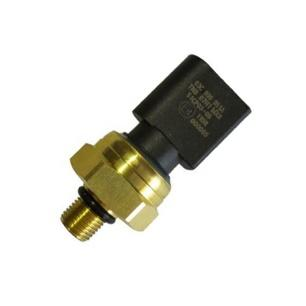
\includegraphics[width=.85\textwidth,height=.60\textheight,keepaspectratio]{figures/ivevo/image21.jpg}
\caption{Давление масла (Barometer)}
\end{figure}
\section{Температура (Thermo)}
Выберите NTC или цифровой DS18B20 и соответствующий скрипт. Поддерживаются кабельные зонды DS18B20. Для NTC рекомендуется Ossca 01176 или совместимый датчик Golf 2. У датчика Ossca соедините контакты датчика 1 и 2; сопротивление NTC подключается к контакту датчика 3. Это номера контактов датчика, а не питания индикатора.

\begin{figure}[H]
\centering
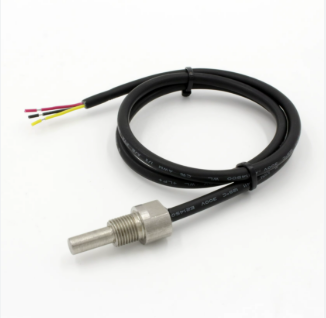
\includegraphics[width=.85\textwidth,height=.60\textheight,keepaspectratio]{figures/ivevo/image14.png}
\caption{Температура (Thermo)}
\end{figure}

\begin{figure}[H]
\centering
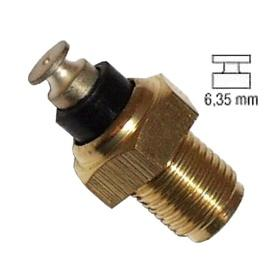
\includegraphics[width=.85\textwidth,height=.60\textheight,keepaspectratio]{figures/ivevo/image19.jpg}
\caption{Температура (Thermo)}
\end{figure}
\section{Индикатор передачи}
Поддерживаются R и передачи 1–5. Передача вычисляется по скорости и оборотам, получаемым от Digifiz Next через Bluetooth LE. Для заднего хода требуется положительный сигнал на входе согласно схеме. Необходима прошивка Digifiz Next 1.0.14 или новее.

Для этого приложения подключите контакт 1 (K30/KL30) к +12 В KL15 после замка зажигания, контакт 7 — к массе. При запуске прочерк означает, что передача не выбрана; устройство ищет Digifiz Next. В режиме QR выберите приложение iv\_gear и датчик volts1, сохраните и перезапустите зажигание.

В веб-панели Digifiz Next откалибруйте скорость по GPS, обороты и таблицу передач под автомобиль. Источник предлагает 80–100 км/ч как опорную скорость: измеряйте только в безопасных и разрешённых условиях, запись поручите пассажиру. Для значений калибровки оборотов 1500, 3000 и 400 не указаны однозначные единицы или соответствие двигателям. Используйте инструкцию приборной панели для конкретного двигателя, не подбирайте значения наугад.

\begin{figure}[H]
\centering
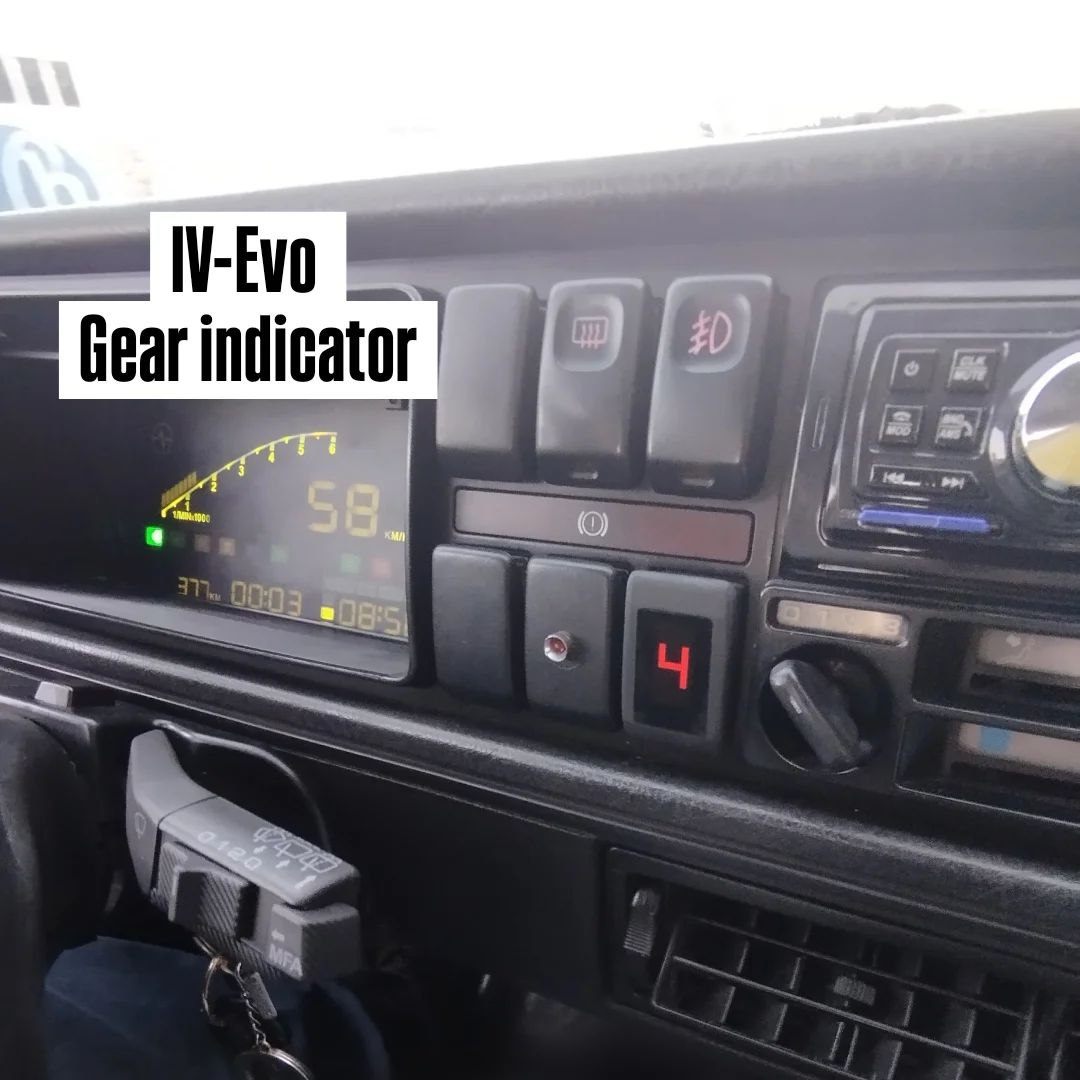
\includegraphics[width=.85\textwidth,height=.60\textheight,keepaspectratio]{figures/ivevo/image18.png}
\caption{Индикатор передачи}
\end{figure}

\begin{figure}[H]
\centering
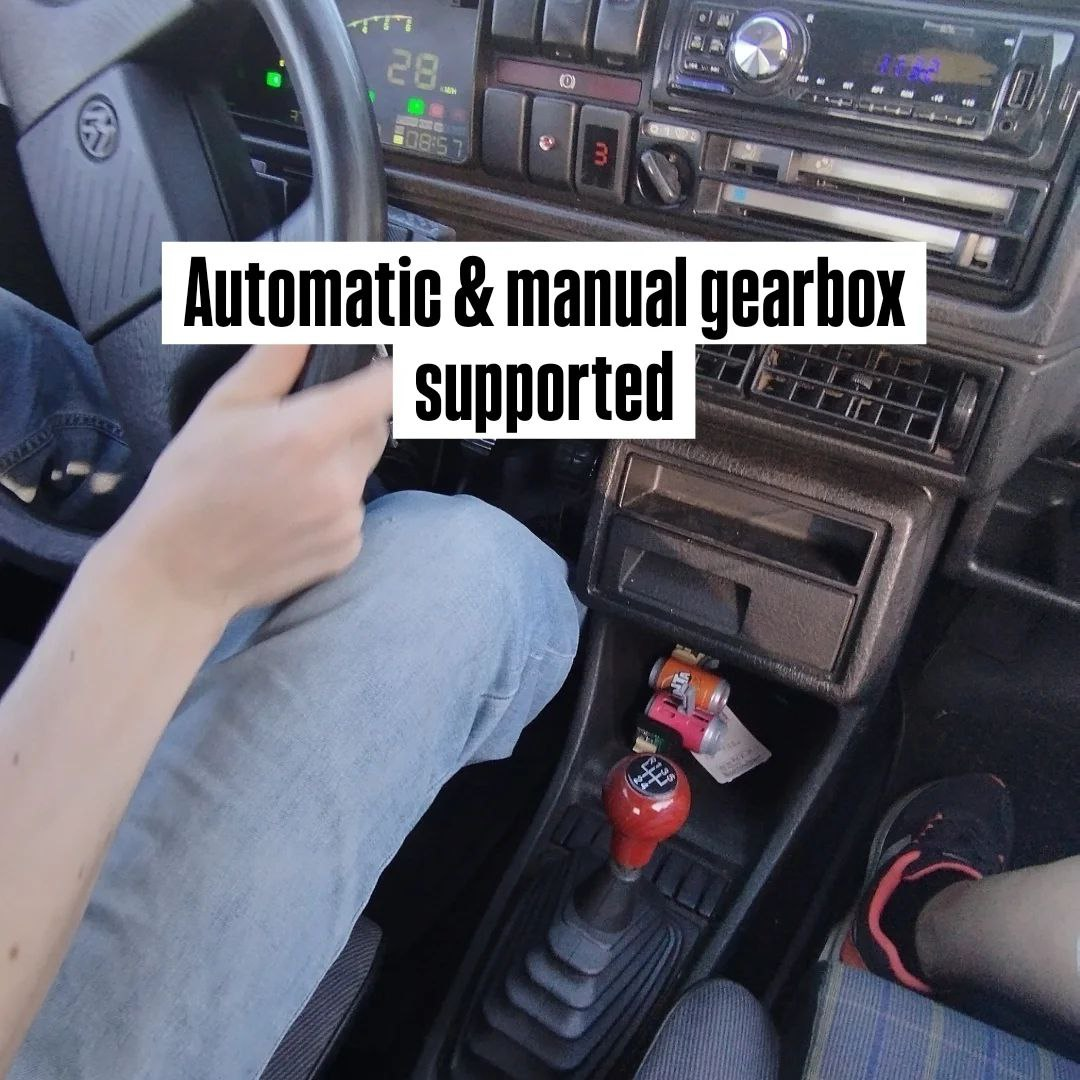
\includegraphics[width=.85\textwidth,height=.60\textheight,keepaspectratio]{figures/ivevo/image10.png}
\caption{Индикатор передачи}
\end{figure}
\section{Лямбда}
Не подключайте индикатор к штатной лямбда-сонде Golf 2. Источник требует отдельную измерительную сонду; при сохранении штатной в автомобиле будет две сонды. Узкополосная сонда даёт примерно 0,1 В для бедной и 0,9 В для богатой смеси, но не измеряет точное соотношение воздуха и топлива. Прямое подключение требует калибровки.

Широкополосной сонде нужен отдельный контроллер: IV-Evo не может управлять ею напрямую. Рекомендуется Bosch LSU 4.9 с совместимым контроллером, например SLC Free, DIY-EFI TinyWB, Sigma Lambda Controller Free 2 или rusEFI wideband. Подключите сонду по инструкции контроллера и используйте его аналоговый выход. Он может иметь диапазон 0–5 В, 0,5–4,5 В или 0–1 В; преобразование входа и калибровочная кривая должны соответствовать ему.

\begin{figure}[H]
\centering
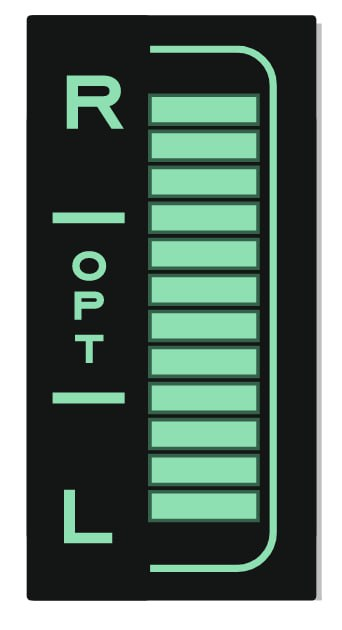
\includegraphics[width=.85\textwidth,height=.60\textheight,keepaspectratio]{figures/ivevo/image7.png}
\caption{Лямбда}
\end{figure}
\section{Check Engine}
При 12 В на контакте 2 (V2) отображается «Check Engine», при 0 В экран пуст. Это индикатор сигнала; чтение кодов неисправностей или интерфейс OBD не описаны.

\begin{figure}[H]
\centering
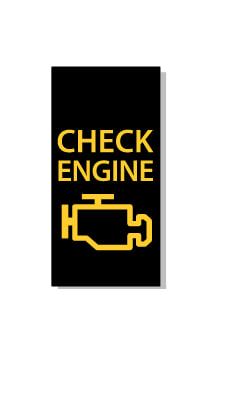
\includegraphics[width=.85\textwidth,height=.60\textheight,keepaspectratio]{figures/ivevo/image4.png}
\caption{Check Engine}
\end{figure}
\section{Наддув (Boost)}
Описан трёхконтактный датчик с питанием +5 В, одним крепёжным отверстием и диапазоном 20–250 кПа. Номинальный выход составляет +1,8 В. Соответствующее давление и полная передаточная функция не приведены. До калибровки уточните точный датчик и его характеристику; не определяйте наклон по одному значению.

\begin{figure}[H]
\centering
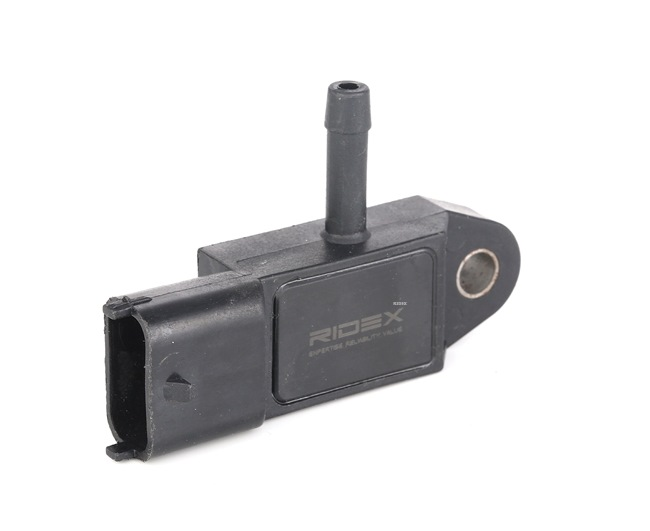
\includegraphics[width=.85\textwidth,height=.60\textheight,keepaspectratio]{figures/ivevo/image9.png}
\caption{Наддув (Boost)}
\end{figure}
\section{Часы}
Приложение-пример использует системные часы. Время не сохраняется после перезапуска; без повторной установки приложение работает как счётчик времени поездки.

\begin{figure}[H]
\centering
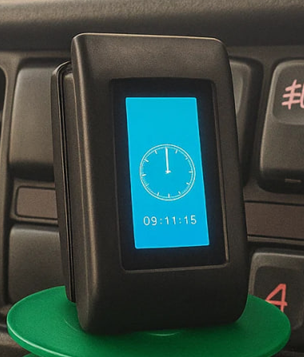
\includegraphics[width=.85\textwidth,height=.60\textheight,keepaspectratio]{figures/ivevo/image12.png}
\caption{Часы}
\end{figure}
\section{Ограничения документации}
Общие допуски питания, рабочий температурный диапазон и степень защиты корпуса не указаны. Не переносите характеристики Nano на IV-Evo.
